\begin{song}{title=\predtitle \centering Anděl \\\large Karel Kryl   \vspace*{-0.3cm}}  %% sem se napíše jméno songu a autor
\begin{centerjustified}
\nejnejvetsi
\sloka
	^{G}Z ^{\z Emi}rozmlácenýho kostela ^{G\z}v~krabici ^{D7\z}s~kusem mýdla

	^{G\z}přinesl ^{Emi}jsem si anděla, ^{G{\color{white}\_\_}D7}polámali mu křídla.

	Díval se na mě oddaně, já měl jsem trochu trému,

	tak vtiskl jsem mu do dlaně lahvičku od parfému.

\refren
	^{G\z}A~proto, ^{Emi\z }prosím, věř mi, ^{G\z}chtěl jsem ho ^{D7\z}žádat,

	^{G}aby mi ^{Emi\z }mezi dveřmi ^*{G}po mohl ^*{D7}hád at,

	^{G}co mě čeká ^{Emi} ^{D}a nemine, ^{G}co mě čeká ^{Emi} ^{D7}a  ^*{\z G}nemine .

\begin{minipage}{0.65\textwidth}
\sloka
	^{G\z}Pak ^{ Emi}hlídali~jsme oblohu, ^{G\z D7\,}pozorujíce ptáky,

	^{G\z Emi\:\,}debatujíce~o Bohu ^{G\z}a~hraní ^{D7\z}na~vojáky.

	^{G\z}Do~tváře ^{Emi\z}jsem mu neviděl, ^{G\z}pokoušel ^{D7\z}se~ji schovat,

	^{G\z}to~asi ^{Emi\z}ptákům záviděl, ^{G}že mohou ^{D7\z}poletovat.

\refren
\end{minipage}
\begin{minipage}{0.1\textwidth}
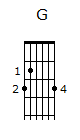
\includegraphics[width=3cm]{../Akordy/g.png}
\end{minipage}

\begin{minipage}{0.65\textwidth}
\sloka
	^{G\z}Když ^{Emi\:\:}novinky~mi sděloval ^{G\z}u~okna ^{D7\z}do~ložnice,

	^{G}já křídla ^{Emi\z}jsem mu ukoval ^{G\z}z~mosazný ^{D7\z}nábojnice,

	^{G\z}a~tak jsem ^{Emi\z}pozbyl anděla, ^{G}on oknem ^{D7\z}odletěl mi,

	^{G\z}však přítel ^{Emi\z}prý~mi udělá ^{G\z}novýho ^{D7}z~mojí helmy.
\end{minipage}
\begin{minipage}{0.1\textwidth}
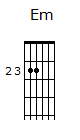
\includegraphics[width=3cm]{../Akordy/em.png}\\
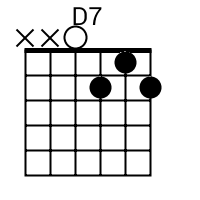
\includegraphics[width=3cm]{../Akordy/d7.png}
\end{minipage}


\refren

\end{centerjustified}
\setcounter{Slokočet}{0}
\end{song}
